% This is a sample document using the University of Minnesota, Morris, Computer Science
% Senior Seminar modification of the ACM sig-alternate style. Much of this content is taken
% directly from the ACM sample document illustrating the use of the sig-alternate class. Certain
% parts that we never use have been removed to simplify the example, and a few additional
% components have been added.

% See https://github.com/UMM-CSci/Senior_seminar_templates for more info and to make
% suggestions and corrections.

\documentclass{sig-alternate}
\usepackage{color}
\usepackage[colorinlistoftodos]{todonotes}

%%%%% Uncomment the following line and comment out the previous one
%%%%% to remove all comments
%%%%% NOTE: comments still occupy a line even if invisible;
%%%%% Don't write them as a separate paragraph
%\newcommand{\mycomment}[1]{}

\begin{document}

% --- Author Metadata here ---
%%% REMEMBER TO CHANGE THE SEMESTER AND YEAR AS NEEDED
\conferenceinfo{UMM CSci Senior Seminar Conference, December 2017}{Morris, MN}

\title{Point-of-Interest Recommendation Systems in Location-Based Social Networks}

\numberofauthors{1}

\author{
% The command \alignauthor (no curly braces needed) should
% precede each author name, affiliation/snail-mail address and
% e-mail address. Additionally, tag each line of
% affiliation/address with \affaddr, and tag the
% e-mail address with \email.
\alignauthor
Myeongjae Song\\
	\affaddr{Division of Science and Mathematics}\\
	\affaddr{University of Minnesota, Morris}\\
	\affaddr{Morris, Minnesota, USA 56267}\\
	\email{songx823@morris.umn.edu}
}

\maketitle
\begin{abstract}
``TBA"
\emph{This will be gone (hopefully)}

% The current paper format *only* allows inline comments using the todo
% macro. That's kind of a bummer, and it would be neat if someone figured
% out how to change the acmconf style to allow this. I suspect it isn't *hard*
% but there are quite a few details that have to be sorted out in synchrony.
\todo[inline]{Needs more work}
\end{abstract}

\keywords{Recommendation Systems, Point-of-Interest Recommendation, Location-Based Social Networks}


\section{Introduction}
\label{sec:introduction}

Nowadays, location-based social networks (LBSN), such as \emph{Facebook places, Tinder},  and \emph{Yelp}, 
have been gaining a lot of attention with the widespread use of smartphones embedded with the 
global positioning system (GPS). Even though LBSN are relatively new compared to 
the traditional social networking services, millions of active users use the platform on a daily basis voluntarily sharing 
their location information. Many of these LBSNs allow users to ``check-in" 
places like a restaurant or cinema; we call these checked-in places the points of interest (POI) 
of the users. Users can share videos, pictures, or reviews about the places via this ``check-in" 
feature. Based on the collected user data, LBSNs provide POI recommendations. POI recommendation 
is very important for LBSNs for two reasons. First, users are more likely use the platform and check-in places 
for their own benefit if it gives accurate predictions on places where users visit next time. 
Second, it allows the advertisers launch advertisements for target user groups. Therefore, 
accurate POI recommendation is crucial for the success of LBSNs.

Even though POI recommendation is a type of recommendation system, it has distinct characteristics 
mainly due to its geographical nature. For instance, recommending a movie is a fairly different task from 
recommending a place. A movie recommendation system can recommend any movie, but a POI recommendation 
system should not just recommend a sushi restaurant in Tokyo for a user in Minnesota. The following are 
meaningful differences between conventional recommendations and POI recommendation:

\begin{itemize}
\item[--] The types of checked-in place are highly related to the time period. Figure \ref{fig:NYC_checkIn} shows check-in data in 
NYC from a LBSN (Foursquare) over different hours of a day. The number of check-ins clearly varies depending 
on the time.
\item[--] People are likely to visit nearby places because of geographical limitation. Not many people are willing 
to fly to Japan from the US just for a nice sushi restaurant.
\item[--] The transition between POI is strongly affected by the user's own preference. Li et al. [2017] refers this as a long-term individual preference. For instance, some people go to the gym after work, but some people go home right away after work. 
\item[--] A user's next location is highly related to the user's current location. We would call this the sequential feature of POI recommendation. 
\end{itemize}

\begin{figure}
\centering
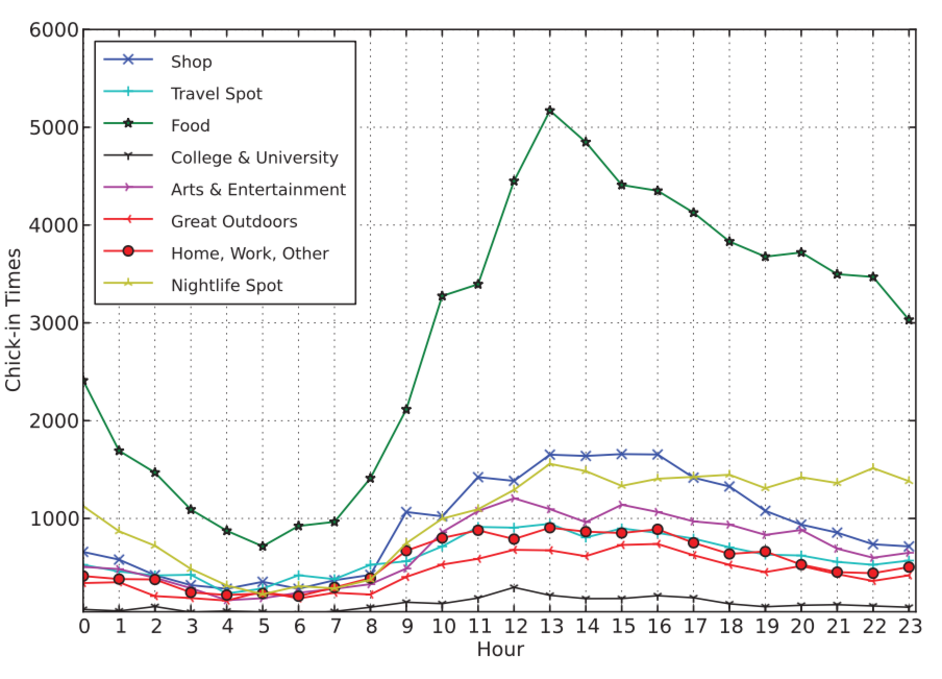
\psfig{file=NYC_checkIn.pdf,width=3.5in}
\caption{Relationship between time interval and check-in location category in NYC.}
\label{fig:NYC_checkIn}
\end{figure}

Traditionally, matrix factorization (MF) or Markov chain (MC) have been popular techniques for producing recommendations.
The ideas behind MF and MC will be explored in more detail in section \ref{sec:backgrounds}. 
Because of the known drawbacks of each model, Rendle et al. [2010] proposes factorizing personalized 
Markov chains (FPMC), which is the combination of MC and MF techniques. FPMC is a robust system, 
but it is a generic model and not designed for POI recommendations. To capture the locality feature of 
POI recommendations, Cheng et al. [2013] suggests FPMC-LR method where LR stands for localized regions. 
And, Li et al. [2017] proposes time-aware FPMC with time decaying consideration called TAD-FPMC.

In section 2, we are going to cover general and mathematical backgrounds in recommendation systems 
to understand the proposed models. Then in section 3, we will explore the proposed approaches in detail. 
In section 4, we will compare the accuracy of different recommendation techniques: FPMC, FPMC-LR, and TAD-FPMC. 
Finally, we will conclude the paper in section 5.

\begin{figure}
\centering
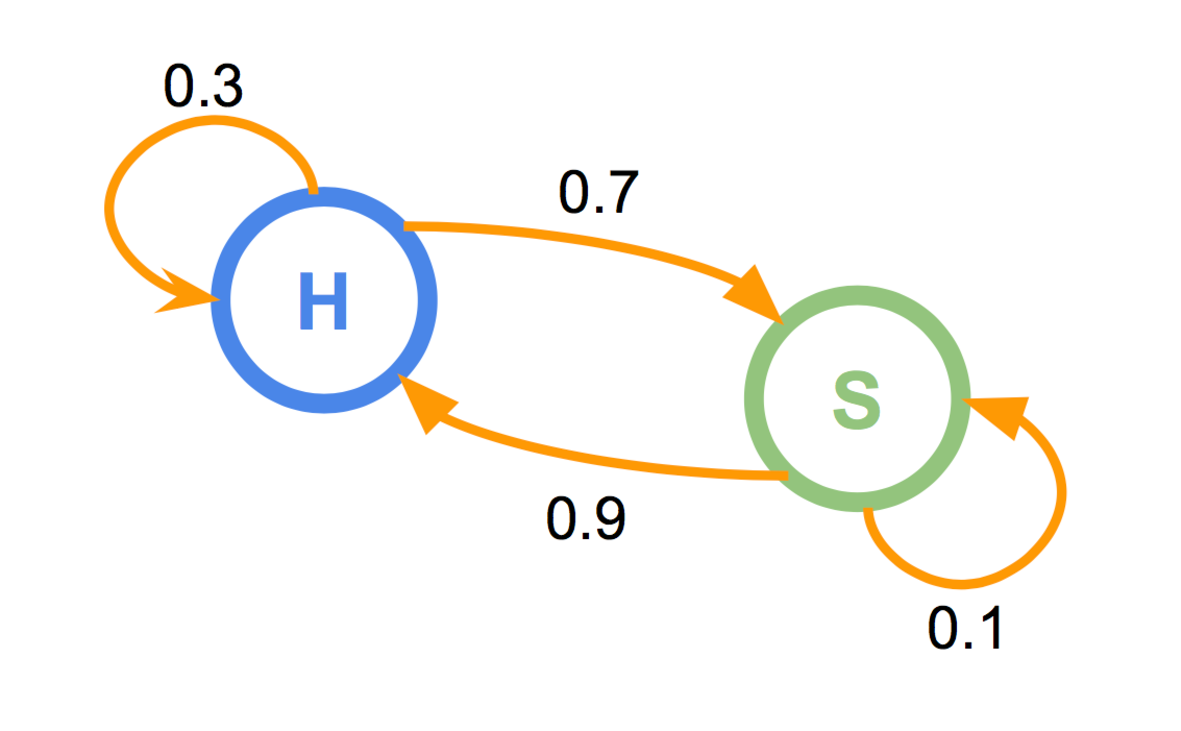
\psfig{file=MarkovChain.pdf,width=3in}
\caption{Markov chain with two states H (house) and S (school)}
\label{fig:MarkovChain}
\end{figure}

\section{Backgrounds}
\label{sec:backgrounds}

\textbf{Markov chain.} Markov chain is a statistical model that represents transitional probabilities among different states. 
In other words, it is a map of transitions from one state to another state. In the context of LBSN, 
states represent different locations where users can visit. Figure \ref{fig:MarkovChain} shows a simple Markov chain 
model with two possible states: house (H) and school (S). The number labels on arrows represent 
the probability of the transition to the indicated direction. In the figure, if the current state of the 
user is H, the probability of the user going to S (going to school) is 70\% and the probability of the 
using going to H again (staying at home) is 30\%. The diagram of states and transitions can also be 
represented as a transition matrix, which allows the mathematical analysis. One key 
feature of the Markov chain is that predictions of future transitions are solely based on the present 
system. Therefore, the previous iterations and future iterations are completely independent. 
Just like the simply example above, we can easily imagine that Markov chain is directly applied to 
POI recommendation systems but with tens of thousands of places instead of two places.

\textbf{Matrix factorizaion.} In Linear Algebra, matrix factorization (MF) is a technique to factor a matrix as a product of multiple matrices. 
When it is used in LBSN context, a realistic example would be a matrix of user x location 
where each entry is the 5 star-based rating of the place like figure *. MF will factor this matrix 
into two separate matrices, one for users and one for the locations. In this factorization, the 
choice of d matters for its efficiency and accuracy, so it should be carefully chosen. Also, 0 
entries are ignored in the factorization stage. With these two factored matrices, we can 
calculate the predicted rating of the place p for user u: 

\textbf{Tensor.} A tensor is essentially a quantity which can represented by a magnitude, a direction, and 
a dimension. Remember a vector is a quantity of a magnitude and a direction, and a scalar 
is a quantity of a magnitude. So, a vector is actually a tensor of rank 1 and a scalar is a tensor 
of rank 0. Simply put, a rank 2 tensor can be represented as a matrix, and higher rank tensors 
are thought as multi-dimensional version of the matrix. For instance, we can stack matrices on 
the top of one another to represent a 3 rank cube-shaped tensor. Figure * shows the visual representations of these tensors.


\section{Factoring Personalized Markov Chain and its improvements}
\label{sec:fpmc}

As we have discussed in section \ref{sec:backgrounds}, MC and MF based recommender systems
have fairly distinct characteristics from each other. In this section, we will study a model called 
Factoring Personalized Markov Chain (FPMC) that incorporates MF into MC, and then its 
enhancements specializing in LSBN data properties.

\subsection{Formalizaion}
\label{sec:typeChangesSpecialChars}

Before we dive into the details, let us introduce the notation used in this paper. 
Let $U$ be a set of users and $L$ be a set of locations. For each user $u \in U$, 
we know their check-in history set \begin{math}L^t_u\end{math} where $t$ is a timestamp 
of the user visit. Our goal now is given the user check-in data 
\begin{math}L^1_u,...,L^t_u\end{math}, recommend a next location to 
a user $u$ at time $t + 1$.

\begin{figure*}
\centering
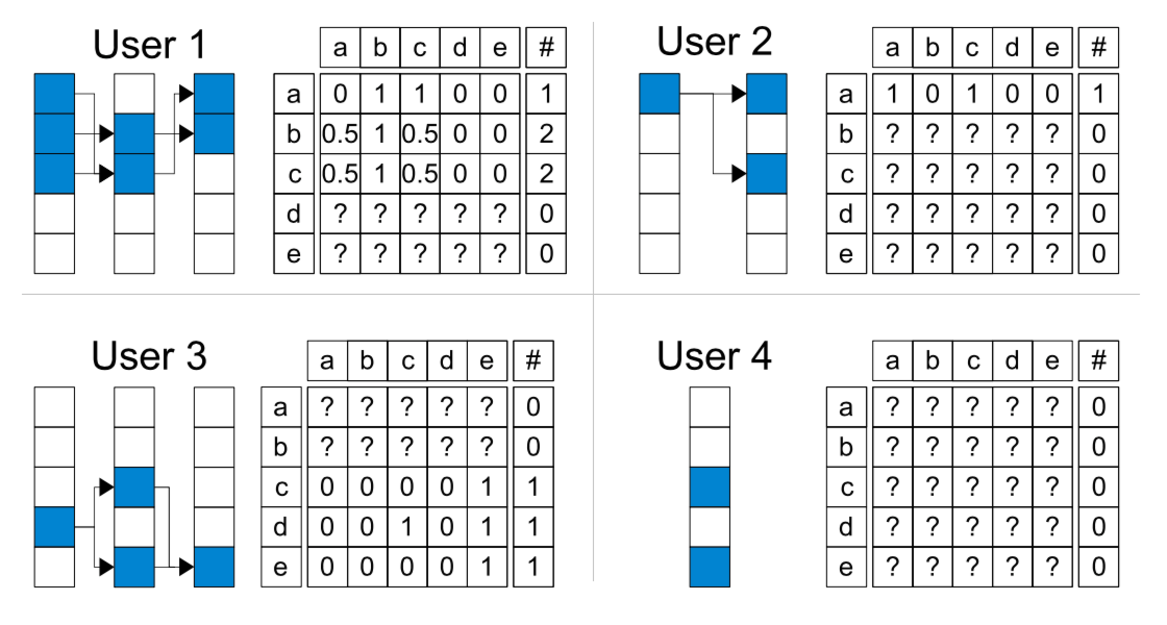
\psfig{file=FPMC_naive.pdf,width = 5in}
\caption{Personalized Markov chains.}
\label{fig:FPMC_naive}
\end{figure*}

\begin{figure}
\centering
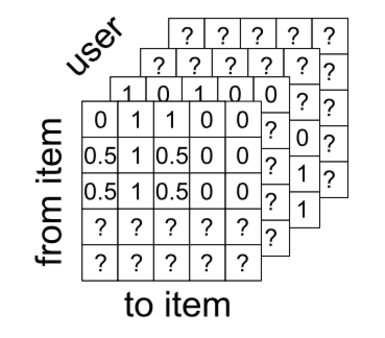
\psfig{file=FPMC.pdf,width= 2in}
\caption{Personalized transition tensor.}
\label{fig:FPMC}
\end{figure}

\subsection{FPMC}
\label{sec:typeChangesSpecialChars}

Even though MC based recommender systems were widely studied and used because of 
its capacity to capture sequential data, it lacks the personalization feature to distinguish each user. 
MF also has its weakness in processing sequential information since it often ignores
 the individual user's preference. The weakness is particularly problematic in LBSN. 
As we have looked at in section \ref{sec:introduction}, sequential information plays a huge role in LBSN 
in that there is a strong connection between recently visited locations and future locations. 
A recommender system with no sequential awareness 
may recommend another restaurant to a user who just check-ined a restaurant; this is not ideal. 
To take advantage of both MF and MC models, Rendle et al. [2010] proposes factorizing personalized 
Markov chains (FPMC).

How does FPMC combine these two different techniques? The most straightforward solution that 
we can think of is having a personalized MC per user $u \in U$. Figure \ref{fig:FPMC_naive} shows 
four different transition matrices for each user. 
? entries mean we have no data 
to estimate the probability of the transition. As we can observe from the matrices, simply using 
personalized transition matrices produces poor estimations. We just do not have enough data from
each user. This is the place where the ideas of 
MF can be applied. By stacking all transition matrices of users, we can get a transition cube or tensor $A$. 
This is the essence of FPMC. Figure \ref{fig:FPMC_naive} represents the tensor for the same data from figure 
\ref{fig:FPMC}. Unlike the naive personalization MC approach, a factored tensor solves the sparsity problem and 
still has its personalization feature for individual users.

\subsection{FPMC-LR}
\label{sec:typeChangesSpecialChars}

FPMC successfully incorporates the information of the personalized Markov chain 
by combining MF and MC in CF. However, it overlooks another noticeable property 
of the LBSN datasets, localized region constraint. The figure ~\ref{fig:onlyOne}  
reports the distance of inter check-ins in Gowalla and Foursquare. It shows that 
more than 75\% of inter check-ins from Foursquare and 80\% of inter check-ins 
from Gowalla happened within 10 km. Only less than 5\% of inter check-ins occur 
more than 100km both in Foursquare and Gowalla. The observation on the LBSN 
shows the trend that users tend to check in places close to their previous check-ins, 
but the FPMC does not really make use of this potentially useful trend.

To add the ability to use localized region constraint 
information into the existing personalized POI Markov chain, Cheng et al. [2013] 
introduces a model called FPMC-LR which combines FPMC model with localized 
region constraints to provide accurate successive POI recommendation in LBSNs. 
Because FPMC-LR only takes into account nearby candidate locations depending 
on where the users are, it reduces the computational costs and noisy information. 
Also, it results in more accurate predications as we will see in [section result].

FPMC-LR model has a similar setting as FPMC since it is an improvement 
over it. Just like in FPMC, the fundamental goal of FPMC-LR is to give the most suitable 
location recommendation for user $u$ at time $t + 1$, given a sequence of check-ins. 
In other words, we need to calculate the probability of a user $u$ to visit a location $l$ at time $t$:
\begin{equation}
	x_{u,i,l}=p(l \in L_u^t | i \in L_u^{t-1})
\label{eq:summation}
\end{equation}
The main difference between FPMC and FPMC-LR is in their transition tensor. As we saw earlier, in FPMC, the model takes into account all possible locations for each user, so the tensor looks like: 
\begin{equation}
	\chi \in [0, 1]^{|U| \times |L| \times |L|}
\label{eq:summation}
\end{equation}
In FPMC-LR, the model only considers neighbor locations for each location l for each user. 
The tensor transition in FPMC-LR looks like:
\begin{equation}
	\chi \in [0, 1]^{|U| \times |L| \times |N_d(L)|}
\label{eq:summation}
\end{equation}
The neighbor locations \begin{math}N_d(L)\end{math} are calculated by Haversine formula, 
which is used to find the shortest distance between two points on the surface of a sphere. 
In this case, we assume the earth is a roughly sphere. After applying several steps of ranking techniques, 
we can get the final probability \begin{math}x_u,t,l\end{math}.

\subsection{TAD-FPMC}
\label{sec:typeChangesSpecialChars}

FPMC-LR is a very successful model for POI recommendation in terms of performance and efficiency 
as we will discuss in later section; it incorporates sequential data with personalization and locality consideration. 
However, there is a still room for improvement. Li et al. [2017] points out that FPMC-LR approach simply captures 
the consecutive ordering relations in lieu of considering complex user behavior over time. Take college students, 
for example. Students have morning classes, afternoon classes, or both in one day. When they have morning classes, 
some of them have breakfast at a brunch cafe after class. When they have afternoon classes, some of them go 
for a drink at a bar after class. Simply combining them as one sequential pattern is clearly not sufficient (e.x. recommending 
for a drink at a bar after 8:00AM class). In other words, just recognizing sequential data is not 
enough for capturing the differences in regular periodic pattern.

To make the system consider users' time-varying behavioral trends, Li et al. [2017] suggests time-aware FPMC (TA-FPMC) 
model, which is an improvement over FPMC-LR model. In section 2-1, Rendle et al. [2010] uses third order tensor to 
construct a personalized Markov chain. TA-FPMC takes a similar approach. Instead of a third order tensor of 
user-location-location, it forms a fourth order tensor by adding a time factor. Now, the transition tensor looks like: 
\begin{equation}
	\chi \in [0, 1]^{|U| \times |T| \times |L| \times |L|}
\label{eq:TA-FPMC_tensor}
\end{equation}
There is another statistical characteristic of LBSN data that has not got much attention, the time gap between 
two successive check-ins. The LBSN data shows that many of two successive check-ins span a large time gap 
like a year. Base on the assumption that these successive check-ins with large time gaps do not tell much, 
Li et al. [2017] introduces another factor $D(\Delta t)$ to take into account the time-decaying effect. 
The final model with all the considerations is called TAD-FPMC.

\section{Experiments}
\label{sec:experiments}
In the experiments, we will address the following questions: 1) How do the different POI recommendation 
models perform in real LBSN data? 2) Why are distance constraint and temporal information important 
factors in POI recommendation?

\subsection{Datasets}
\label{sec:datasets}
The evaluation used data collected from Foursquare, a LBSN that provides POI recommendations based on 
each user's preference. The data includes users' check-in data of New York City and Los Angeles from Jan. 
2010 to June 2011. Li et al. [2017] divided available locations in the data into 249 categories. 
The summary of the statistics is elaborated in Table 1. In Table 1, \emph{tip} means comments or reviews on a 
certain location written by other users.

\subsection{Evaluation Metric}
\label{metic}
The main task for models is providing a list of top-N locations (the list contains N locations 
ordered from the highest probability of user visit to the lowest). The recommendation is considered 
correct if the user indeed visited a location in the top-N list or the category of the user visit location 
is in the top-N list. The evaluation metric is defined as:
\begin{equation}
	P@N = \frac{\textrm{the counts of correct predictions}} {\textrm{the total number of recommendation rounds}}
\label{eq:P@N}
\end{equation}


\subsection{Comparison}
\label{comparison}
Figure * shows the performance comparison among different models of POI recommendation. 
The x-axis represents the N value which is the number of recommended locations, and the y-axis 
is the precision of the recommendation P@N. In both LA and NYC data, there is a huge gap 
between generic models (MF and FPMC) and POI specific models (FPMC-LR and TAD-FPMC). 
This verifies the importance of distance constraint and temporal information in POI recommendations. 
Also, TAD-FPMC slightly outperforms FPMC-LR in both datasets. If we utilize additional enhancements 
for TAD-FPMC, the performance improves significantly as we can see in Table .

The experiments were run on a machine with a Core i7-6700K 4.0GHz 8HT and memory size of 32GB. 
In terms of the efficiency, TAD-FPMC is shown to be the most efficient model with the running time of 
3 hours compared to FPMC and FPMC-LR with 35 hours. The reduced dimensionality from the number of 
locations to the number dimensionality improves the efficiency significantly.

\section{Conclusions}
\label{sec:conclusions}

TBA

\section*{Acknowledgments}
\label{sec:acknowledgments}

This section is optional; it is a location for you
to acknowledge grants, funding, editing assistance and
what have you.

You want to use the \texttt{\textbackslash section*} version of the \texttt{section}
command, as an acknowledgments section typically does \emph{not} get
a number.

It is common (but by no means necessary) for students to thank
their advisor, and possibly other faculty, friends, and family who provided
useful feedback on the paper as it was being written.

In the present case, for example, the
authors would like to thank Gerald Murray of ACM for
his help in codifying this \textit{Author's Guide}
and the \textbf{.cls} and \textbf{.tex} files that it describes.

% The following two commands are all you need in the
% initial runs of your .tex file to
% produce the bibliography for the citations in your paper.
\bibliographystyle{abbrv}
% sample_paper.bib is the name of the BibTex file containing the
% bibliography entries. Note that you *don't* include the .bib ending here.
\bibliography{sample_paper}  
% You must have a proper ".bib" file
%  and remember to run:
% latex bibtex latex latex
% to resolve all references

\end{document}
